\section{Simulationsbeispiel}
Die vorgestellten Methoden zur lokalen Stabilitätsanalyse eines Netzwerks werden in diesem Abschnitt auf ein Beispiel angewendet. Bisher wurden nur dynamische Systeme mit kontinuierlichen Variablen betrachtet. Die zugrunde liegende Theorie lässt sich auch auf diskrete Systeme anwenden. Dabei ist die Dynamik nicht durch ein Differentialgleichungssystem gegeben, sondern durch eine Iterationsvorschrift. Das hier betrachtete Netzwerk \cite{pecora2014} folgt der Dynamik in Gleichung \ref{eq:bspdyn}.
\begin{align}
\label{eq:bspdyn}
	x_i^{t+1}&=\left[\beta\mathcal{I}(x_i^t)+\sigma \sum_j^N A_{ij}\mathcal{I}(x_j^t)+\delta\right] \text{mod}\quad 2\pi
	\\\notag & \beta,\sigma \text{ Kopplungsparameter}
	\\\notag  & \delta \text{ Offset}
	\\\notag &\mathcal{I}(x)=\frac{1-Cos(x)}{2}
\end{align}
Die betrachteten Netzwerke sind symmetrisch und bestehen aus $N=11$ Knoten  (Abb. \ref{fig:cluster}). Die verwendeten Kopplungsmatrizen sind Pecora et al. \cite{pecora2014} entnommen und in Abb. \ref{fig:abmat} dargestellt (siehe auch Anhang). 
\begin{figure}
	 \centering
	 \subfloat[Netzwerk 1]{
	 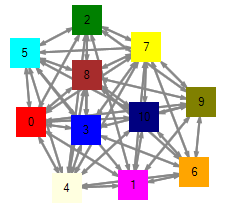
\includegraphics[width=0.25\textwidth]{abb/misc/cluster1.png}
	 }
	 \subfloat[Netzwerk 2]{
	 	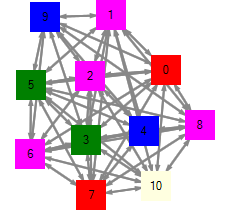
\includegraphics[width=0.25\textwidth]{abb/misc/cluster2.png}
	 }
	 \subfloat[Netzwerk 3]{
	 	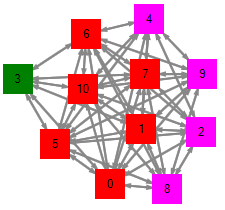
\includegraphics[width=0.25\textwidth]{abb/misc/cluster3.png}
	 }
	 \caption[In der Simulation verwendete Netzwerke]{Die drei verwendeten Netzwerke. Die Knoten eines Cluster sind in der gleichen Farbe eingefärbt.}
	 \label{fig:cluster}
\end{figure}

\begin{figure}
	\centering
	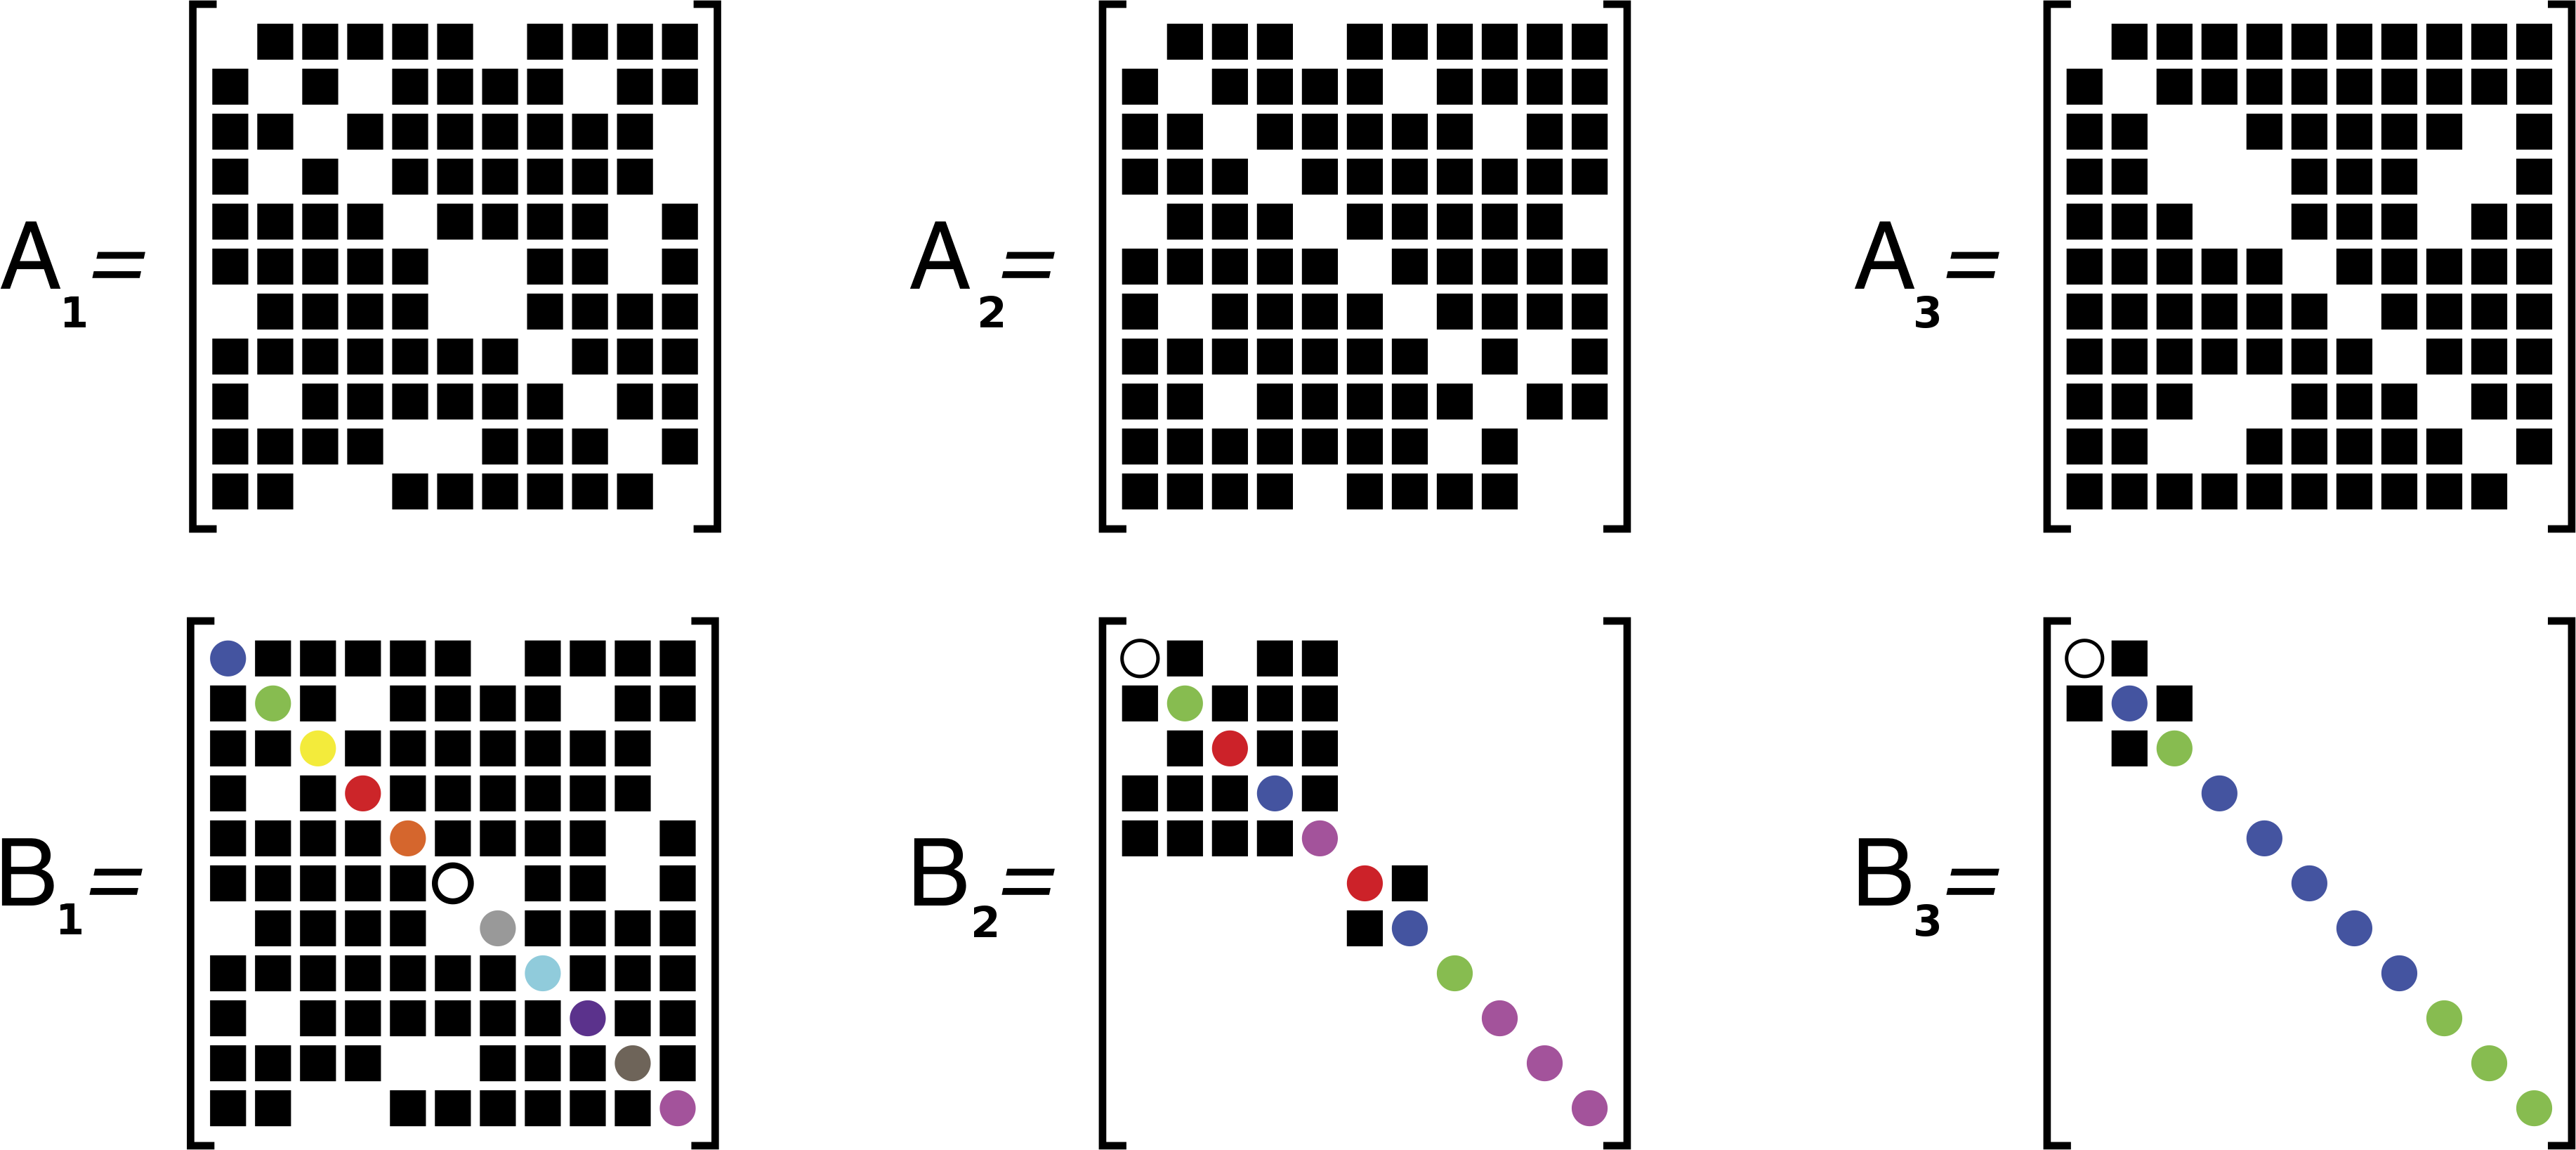
\includegraphics[width=0.75\textwidth]{abb/misc/ABMat.png}
	\caption{Kopplungsmatrizen $\boldsymbol{A}$ der in Abb. \ref{fig:cluster} dargestellten Netwerke sowie die transformierte Kopplungsmatrizen $\boldsymbol{B}$ in der die Zeilen nach den zugehörigen Clustern markiert sind\cite{pecora2014}.}
\label{fig:abmat}
\end{figure}

Für diese Netwerken ergibt die Suche nach Automorphismen der zugrundeliegenden Graphen mit \textit{Nauty} 0, 32 bzw. 5760 Symmetrien und 11 (triviale, nur aus einem Knoten bestehende), 5 bzw. 3 Cluster (Tab. \ref{tab:netzwerke})

\begin{table}[]
	\begin{center}
	\caption{Symmetrien und Cluster der betrachteten Netzwerke}
	\label{tab:netzwerke}
\begin{tabular}{lll}
	Netzwerk & Symmetrien & Cluster                           \\
	\hline
	1        & 0          & 11 triviale Cluster               \\
	2        & 32         & (1,8) (2,3,7,9) (4,6) (5,10) (11) \\
	3        & 5760       & (1,2,6,7,8,11) (3,5,9,10) (4) \\  
	\hline
\end{tabular}
	\end{center}
\end{table}

Zur Berechnung der Ljaponow-Exponenten für die verschiedenen Cluster wurde eine Basistransformation (siehe \ref{stabilitaet}) mit den im Anhang dargestellten Transformationsmatrizen vorgenommen \cite{pecora2014,sagenotebook}.
\begin{figure}
	\centering
	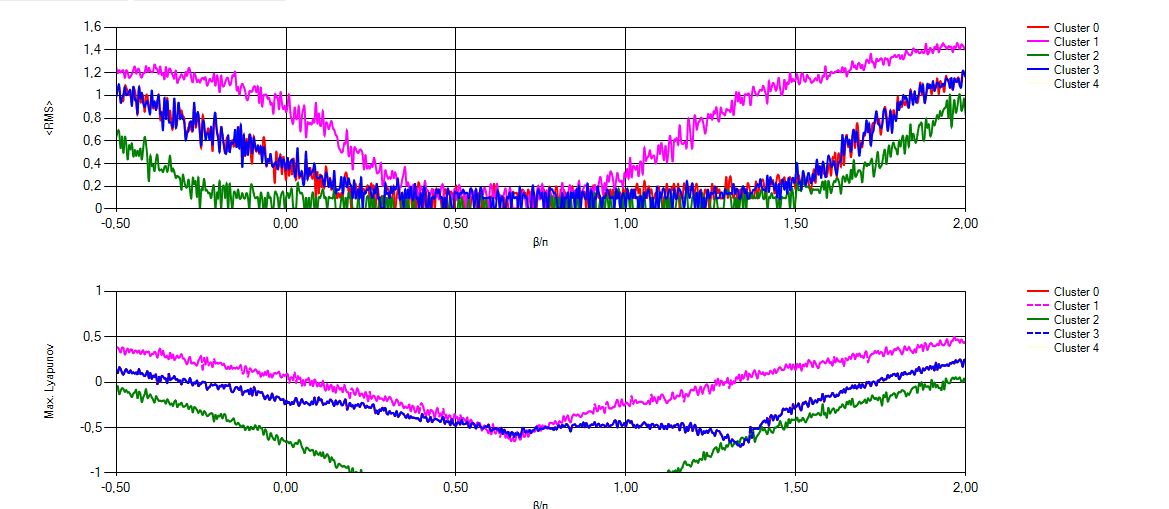
\includegraphics[width=1.0\textwidth]{abb/misc/ljapResult.png}
	\caption{Ergebnisse der Simulation. Die obere Grafik zeigt die mittlere quadratische Abweichung vom Mittelwert für das jeweilige Cluster. Im unteren Bild ist der maximale Ljapunow-Exponent für die Cluster über $\beta$ aufgetragen. Nach einer Transienten von 200 Zeitschritten wurden die mittleren Abweichungen über 1000 weitere Schritte gemittelt.}
	\label{fig:ljapResult}
\end{figure}
Für Netzwerk 1 erübrigt sich aufgrund des Fehlens von Clustern die Stabilitätsanalyse.

Abbildung \ref{fig:ljapResult} zeigt exemplarisch die Simulationsergebnisse für das zweite Netzwerk. Dabei beschreibt RMS die mittlere quadratische Abweichung vom Mittelwert für ein Cluster, also ein Maß für die Asychronizität eines Clusters. Die Anfangswerte $x_i^0$ sind gaußverteilt um $\pi$ mit einer Standardabweichung von 0,01$\pi$ gewählt, also zunächst asynchron. Ein geringes Rauschen von 0,002 ist in jedem Iterationsschritt eingefügt, sodass die Synchronisation zusätzlich gestört wird.

Das RMS geht gegen Null, sobald die MSF negativ ist. Dies stimmt mit den Überlegungen aus \ref{stabilitaet} überein, da die Bahnkurven sich für lange Zeiten wieder annähern, also synchron laufen.
Alle Cluster außer 0 (Rot) und 3 (Blau) weisen eine isolierte Synchronisation auf. Die Synchronisation innerhalb eines Clusters ist unabhängig vom Zustand der anderen. Das blaue und rote Cluster hingegen verlieren (bzw. erreichen) die Synchronizität gemeinsam, sind also interwinded Cluster. Dies wird durch den identischen Verlauf der MSF deutlich.

Analoge Beobachtungen können bei dem dritten Netzwerk gemacht werden. Auch hier verschwindet die Asynchronität der Cluster bei negativer MSF (nicht dargestellt).


